\documentclass{article}
%\usepackage[spanish,activeacute]{babel}
%\usepackage[english,activeacute]{babel}
%\usepackage[latin1]{inputenc}
\usepackage[utf8]{inputenc}
\usepackage[english]{babel}

\usepackage{amsmath,amsfonts,amssymb,amstext,amsthm,amscd}
\usepackage{hyperref}
\usepackage{latexsym}
\usepackage{graphicx}
%\usepackage{subfigure}
\usepackage{subfig}
%\linespread{1.6}
\usepackage{float}
\usepackage{dcolumn}% Align table columns on decimal point(esto lo saque del ejemplo de revtex4)
\usepackage{bm}% bold math(esto lo saque del ejemplo de revtex4)
\newcounter{itemR}
\usepackage{here} %recordar usar el comando[H] para las gráficas que es el comando here en lugar de [h!]
\usepackage{fancyhdr}
%\usepackage{sidecap}
%\usepackage[spanish,activeacute]{babel}
\usepackage{multirow}
\usepackage{multicol}
\usepackage{array}
\usepackage{enumitem}
\usepackage{listings}
%\usepackage{booktabs}% para hacer tablas profesionales con \toprule

% ------------------------------------------------------------------------------------------------------------------------------------------------------

\usepackage{fancyhdr}
\setlength{\headheight}{15.2pt}
\usepackage[paperwidth=8.5in, paperheight=11.0in, top=1.0in, bottom=1.0in, left=1.0in, right=1.0in]{geometry}
\lstnewenvironment{code}{\lstset{basicstyle=\ttfamily}}{}

\pagestyle{fancyplain}
\fancyhead[LE,RO]{Reporte análisis de algoritmos}
\fancyhead[CE,CO]{}
\fancyhead[RE,LO]{O23-LIS2012-1}
\fancyfoot[LE,RO]{\thepage}
\fancyfoot[CE,CO]{Matemáticas discretas, UDLAP}
\fancyfoot[RE,LO]{}

% ------------------------------------------------------------------------------------------------------------------------------------------------------
% ------------------------------------------------------------------------------------------------------------------------------------------------------
\begin{document}
\fancypagestyle{plain}{
   	\renewcommand{\headrulewidth}{1pt}
   	\renewcommand{\footrulewidth}{1pt}
}
\renewcommand{\footrulewidth}{1pt}
\renewcommand{\tablename}{Tabla}
\renewcommand{\figurename}{Figura}

% ------------------------------------------------------------------------------------------------------------------------------------------------------
% ------------------------------------------------------------------------------------------------------------------------------------------------------

\title{Análisis de algoritmos}
\author{\small{Erick Gonzalez Parada ID: 178145}\\
	   \small{Matemáticas discretas, Universidad de las Américas Puebla, Puebla, M\'exico}}
\date{\small{\today}}
\maketitle

% ------------------------------------------------------------------------------------------------------------------------------------------------------
% ------------------------------------------------------------------------------------------------------------------------------------------------------

\begin{abstract}
  El análisis de estos algoritmos de búsqueda\\
permite conocer y empezar a dominar los conceptos del big-o notation\\ 
\\
\\
{\it Keywords:}  búsqueda, algoritmo   
\\
\\
\end{abstract}

% ------------------------------------------------------------------------------------------------------------------------------------------------------

\begin{multicols}{2}
\section{Introducción}\label{Introducción}                              	% -------------------- Introducción
  Primer algoritmo \textit{linear search} se enfoca principalmente en buscar un elemento especifico
  en un array (arreglo) retornando en este caso verdadero si el elemento solicitado se encuentra dentro de este
  y retorna falso si el elemento solicitado no se encuentra en el.\\
  \\
  El segundo algoritmo \textit{binary search} también trata de buscar el elemento solicitado sin embargo función 
  de manera diferente utilizando el concepto de divide y vencerás de tal manera que literal va dividiendo el espacio de búsqueda,
  sin embargo primero el array tiene que estar ordenado ya que lo siguiente después de dividir es preguntar si el elemento solicitado 
  es mayor o menor que la posición en la que se encuentra, a partir de ahí básicamente volvemos a partir hasta que lleguemos a tener dos elementos
  y simplemente preguntaremos si es uno o el otro, si lo encontró regresamos positivo, sino regresamos negativo.
\end{multicols}
\section{Explicación de los algoritmos}\label{explicacion}				% -------------------- Metodología 
A continuación se presentaran los algoritmos con comentarios explicando el pseudocódigo paso a paso\\ 
Nota: en pseudocódigo los comentarios son denotas con un '\%' y no pueden contener acentos.
  \subsection*{linear search}\label{ls}
    \begin{code}
      % Parametros ocupados antes y para que la busqueda lineal funcione
      Requiere: list a, size of list n, desired item x
      % Empieza el primer for loop
      % notar que el for loop esta 0 indexado
        for i=0 to n-1 do
        % si el elemento actual es el que estamos buscando
        % lo retornamos y ahi acaba todo
          if a[i]=x then
            return i
          end if
          % iteramos al siguiente elemento
          i=i+1
        % terminamos for loop
        end for
      % aqui el pseudocodigo esta representando la ultima evaluacion 
      % donde nuestro iterador excede n-1 y con esto indicando que
      % no se encontro el elemento deseado por lo que se retorna falso
      if i=n then
        return false
      end if
    \end{code}

    \subsection*{Binary search}\label{bs}
      \begin{code}
        % Parametros en esta ocacion son tener la lista ordenada 
        % de mayor a menor o de menor a mayor pero tiene que estar
        % ordenada y pues tambien requerimos como parametro al 
        % elemento que deseamos obtener que lo retorna si lo ha encontrado
        % notar que esta vez estamos indexando desde 1 
        binaryS(A[1...n],x)
          % variable entero izquierda apunta al primer elemento
          left = 1
          % variable entero derecha apunta al ultimo elemento
          right = n
            % el siguiente while loop es mientras
            % el valor del ultimo elemento sea mayor
            % o igual que nuestra primer apuntador 
            while(right >= left)
              % un ultimo apuntador
              % que apunta en medio
              % del rango de los valores
              % right & left (floor)
              mid = left + [(right - left)\2]
              % si nuestro apuntador de 
              % en medio ya apunta al
              % elemento deseado 
              % retorna el elemento
              if x = A[mid]
                return mid
              % si no y x es mayor que
              % el elemnto que esta en el
              % medio de nuestro intervalo actual
              % entonces movemos nuestro apuntador de 
              % la izquierda a lo que vale el apuntador
              % de en medio + 1
              if x > A[mid]
                left = mid + 1
              % si no movemos nuestro apuntador de la
              % derecha a lo que vale el apuntador de
              % en medio - 1
              if x < A[mid]
                right = mid - 1
              
            % si no encontramos nada hasta que el while loop da falso
            % retornamos null o bien pues que no encontramos el elemento deseado
            return NULL
      \end{code}
\begin{multicols}{2}
\section{Análisis del algoritmo}\label{AdA}
  Utilizando conteo por bloques se van a analizar ambos algoritmos.
  \subsection*{linear search}
  \begin{figure}[H]
    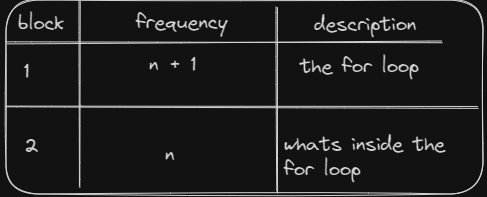
\includegraphics[scale=0.6]{imgs/t0.png}
    \caption{linear search}
    \label{Fig:1}
  \end{figure}
  Función característica: 
  \begin{equation*}
    2n + 1
  \end{equation*}
  Complejidad asintótica
  \begin{equation*}
    O(n)
  \end{equation*}

  \subsection*{binary search}
  \begin{figure}[H]
    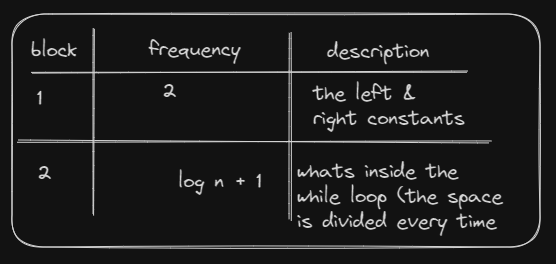
\includegraphics[scale=0.5]{imgs/t1.png}
    \caption{binary search}
    \label{Fig:2}
  \end{figure}

    Función característica
    \begin{equation*}
      2 + \log2 n+1
    \end{equation*}

    Complejidad asintótica
    \begin{equation*}
      O(k + log(n))
    \end{equation*}

    donde k es una constante.

    comparando gráficas donde se quitan las constantes en ambas notaciones asintóticas

    \begin{figure}[H]
      \centering
      \includegraphics*[scale=0.2]{imgs/t2.png}
      \caption{gráficas}
      \label{Fig:3}
    \end{figure}
\section{Conclusiones}\label{Conclusiones}				% -------------------- Conclusiones
Concluyendo es importante reconocer que estas son los algoritmos principales para la búsqueda de algún
elemento y llevándolos a la práctica de la vida real y en lo personal aplicaría linear search en los mínimos casos
en donde se busca un elemento dentro de una lista (o array) pequeño mientras que la búsqueda binaria aplica excelente para cuando
la lista (o array) es de proporciones muy grandes y en la vida real sirve para buscar entre millones de datos.

En otras palabras linear search llega a ser muy poco eficiente en contra de binary search y lo podemos comprobar nuevamente
 viendo la figura \ref{Fig:3}.
\end{multicols}
\end{document}	